\documentclass[14pt,a4paper,pdflatex]{disser}
\usepackage[russian]{babel}
%\usepackage[utf-8]{inputenc}
%\usepackage{amsmath,amssymb}
%\usepackage{longtable}
\usepackage{parskip}
\usepackage{caption}
\usepackage{textcomp}
\usepackage{gensymb}
\usepackage[dvips]{graphicx}
%\usepackage{wrapfig}
%\usepackage{amssymb}*
%\usepackage{color}
%\usepackage{ulem}
\usepackage{setspace}
\usepackage{hyperref}
\usepackage{pdfpages}

\oddsidemargin=-0.5 cm
\evensidemargin=-0.5 cm
\textwidth=170 mm
\textheight=260 mm
\topmargin=0 cm
\voffset= -2cm
\pagenumbering{true}
%\newlength{\varheight}
%\setlength{\varheight}{3.1cm}
\setlength{\parindent}{0cm}
%\newcommand{\taskname}[name]{\begin{center} \bf{\Large{name}} \end{center}}
\spacing{1.1}
\parskip=2mm
\captionsetup[figure]{labelformat=empty}
\clubpenalty=10000
\widowpenalty=10000

\begin{document}

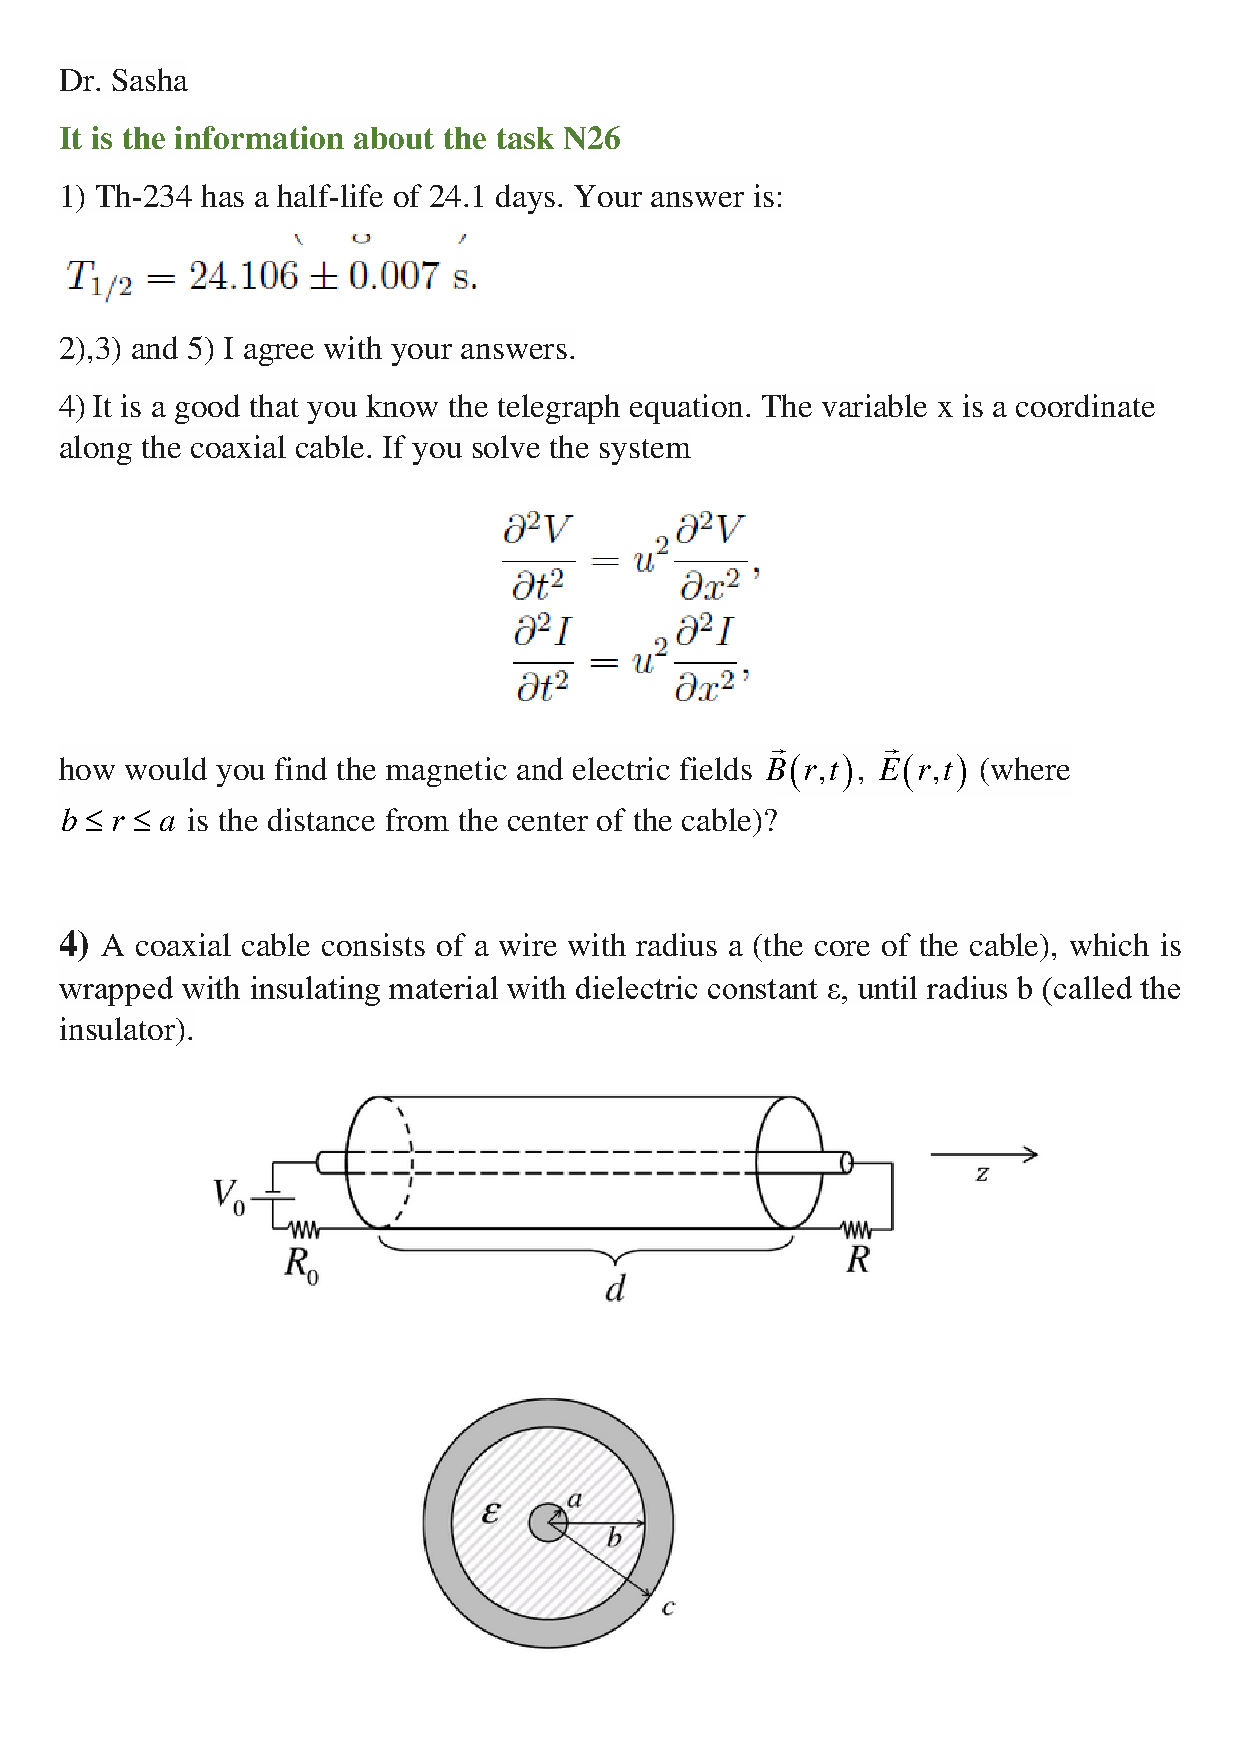
\includepdf{question_for_Sasha26t.pdf}

\pagebreak

1. There may be a misprint, the correct unit is ``days''.

2. With known functions $V(x,t)$ and $I(x,t)$ the fields can be calculated directly from Maxwell equations, e.g. with the method demonstrated in the calculation of the cable's parameters.

\end{document} 